\textbf{$\ket{-} = \frac{1}{\sqrt{2}}(\ket{0}-\ket{1})$}\vspace{.2cm}
\textcolor{bibi}{}
\begin{quote}
    \begin{minted}[fontsize=\small, linenos, frame=single]{python}
circuitoMenos = QuantumCircuit(1)
circuitoMenos.x(0)
circuitoMenos.h(0)
circuitoMenos.measure_all()
circuitoMenos.draw('mpl')
    \end{minted}
    \vspace{.3cm}
    \begin{center}
        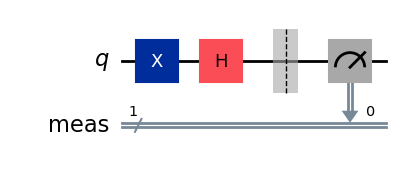
\includegraphics[height=3.3cm]{src/Img/1.3.png}
    \end{center}

    Este es básicamente lo mismo que el anterior pero antes de aplicar H usamos X para
    convertir nuestro \texttt{qubit} en un 1. Después usamos la propiedad: 
    $\hat{H}\ket{1}=\ket{-}$ y terminamos. Al medirlo nos sale lo mismo. 
    \vspace{.5cm}

    \begin{center}
        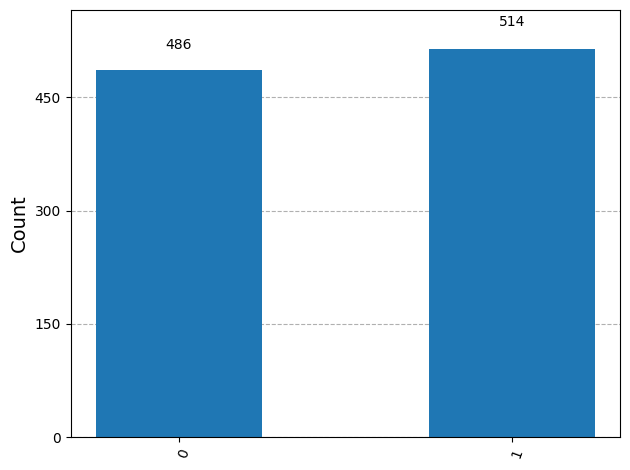
\includegraphics[height=6cm]{src/Img/1.3.r.png}
    \end{center}
\end{quote}
